\chapter{Design Option Structuring Tree}\label{chap:baseline_dot}
The purpose of the design option tree is to find a feasible design option that can satisfy the requirements. This selection process can be an iterative process in case no feasible design option is found in the initial design option tree. By positioning the design options in a tree format, their hierarchical structure becomes visible. The tree is structured such that the most impactful decisions are selected at the top of the tree, whereas more detailed decisions are made at lower levels of the tree. Several subsections are created to  \Cref{fig:baseline_dot} presents the design option tree for this thesis. The nodes in the tree represent design options and child leafs represent design options within a parent design option. For example, a choice may be made to use digital neuromorphic hardware, and within that design space, a particular chip may be selected. Multiple (parallel) design options may be selected. For example, a softwarematic and hardwarematic implementation may be chosen.
\begin{figure}[H]
    \centering
    %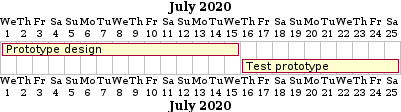
\includegraphics[width=0.6\linewidth]{Images/Diagrams/trivial_gantt.png}
    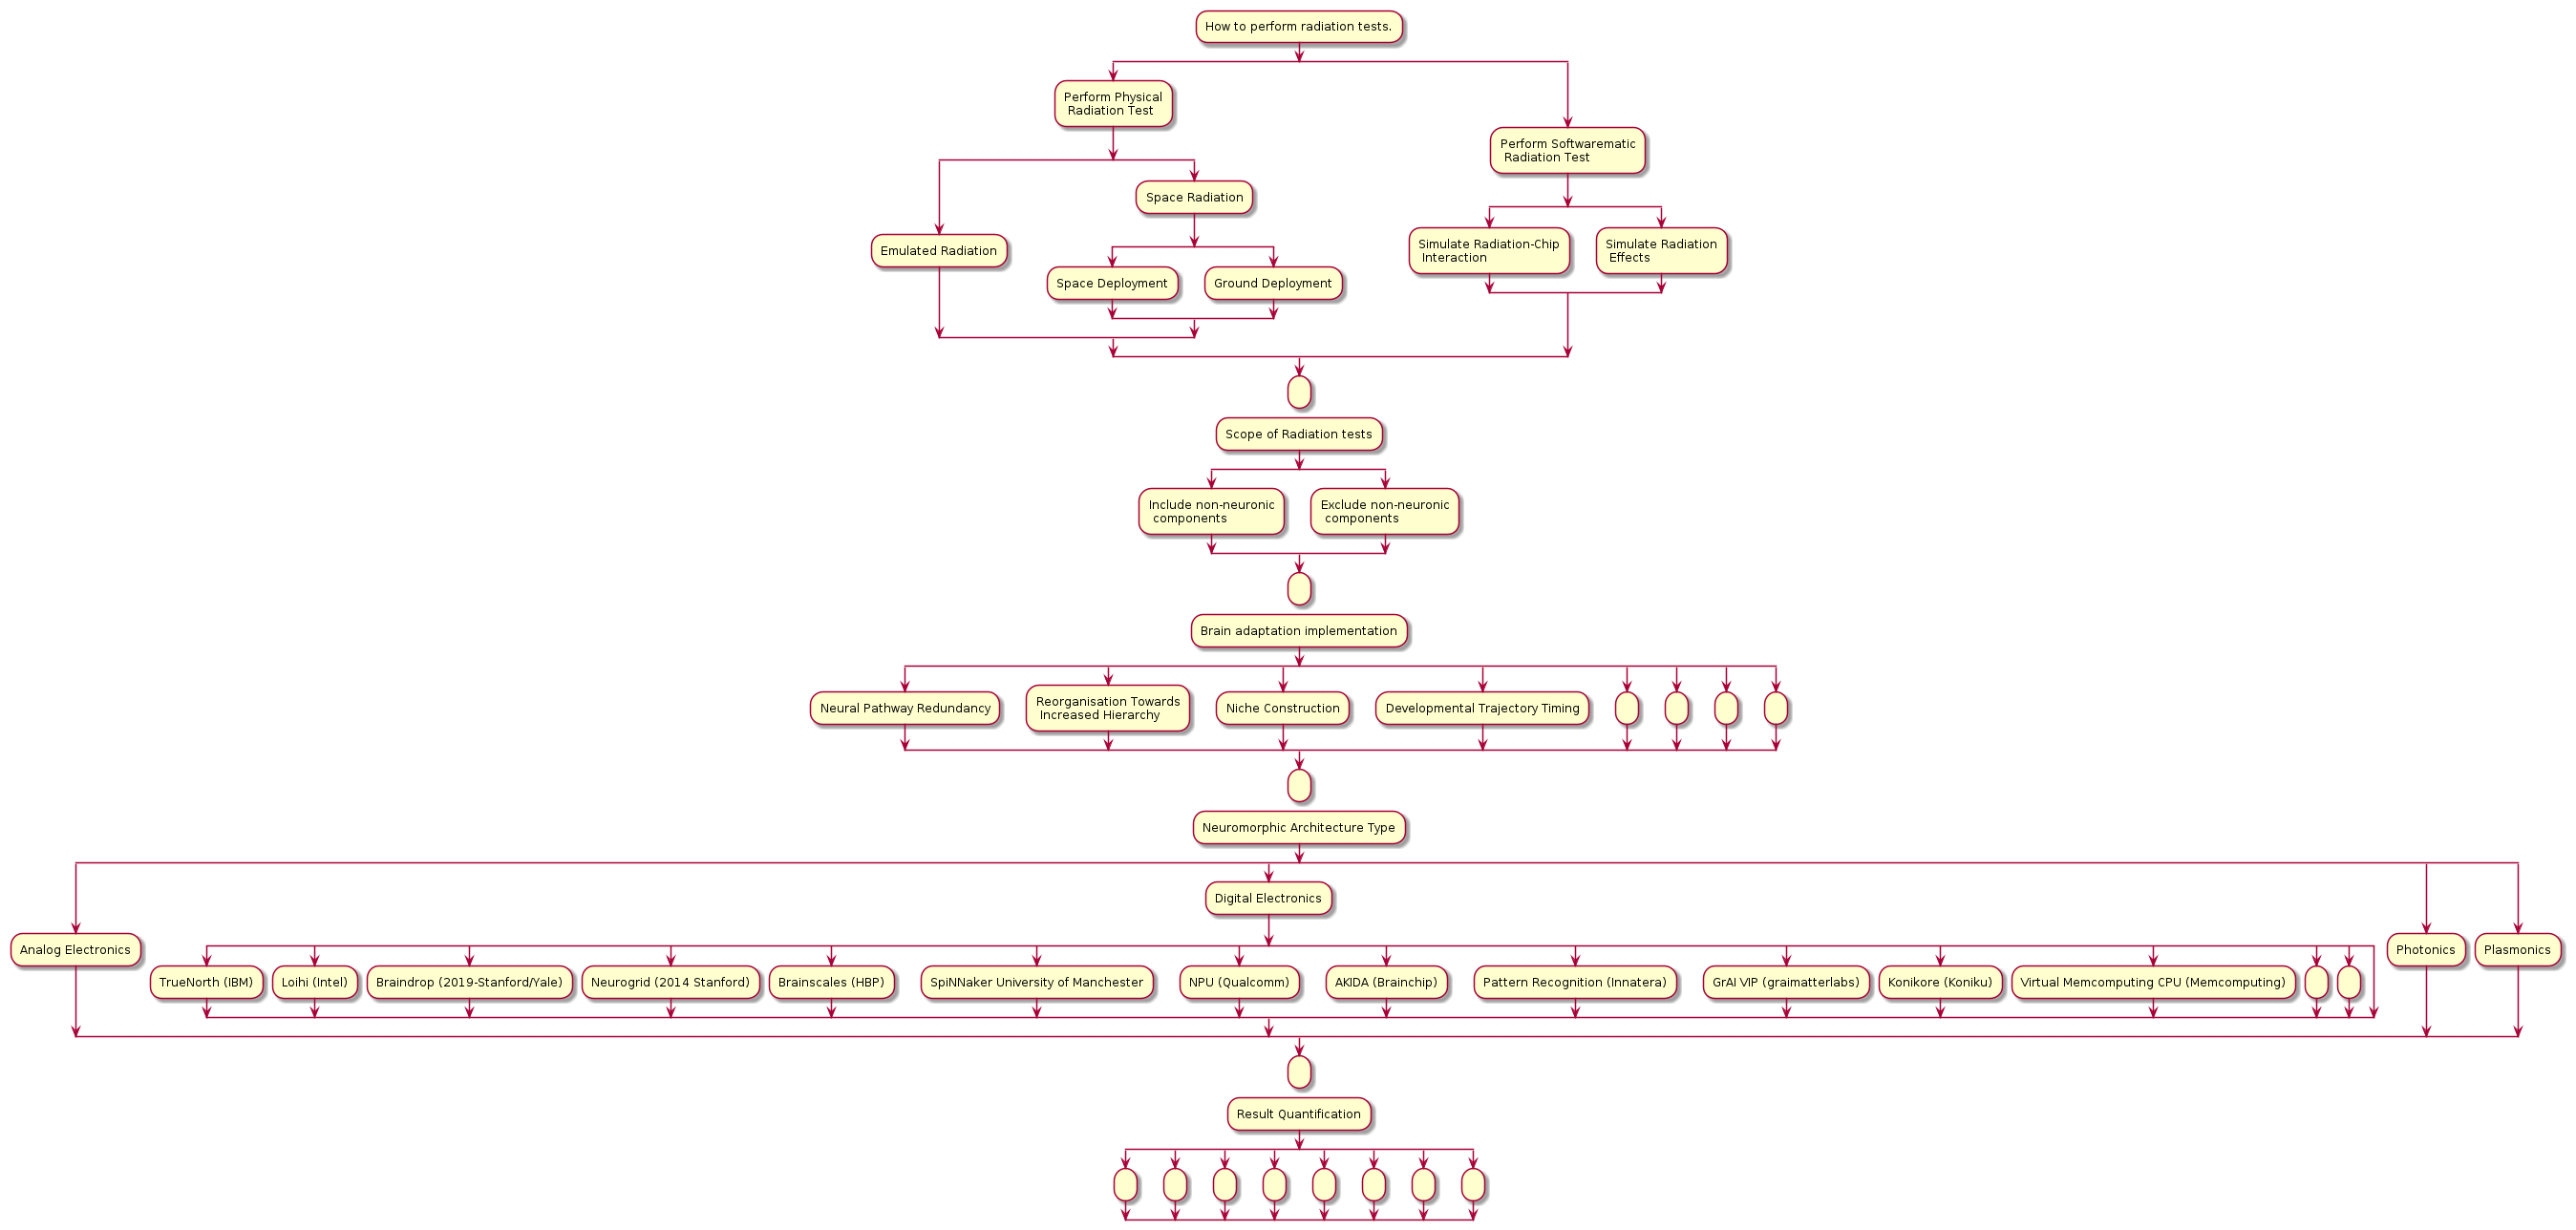
\includegraphics[width=0.6\linewidth]{latex/Images/dot.png}
    \caption{A functional flow diagram with the high-level functions of the system that is to be designed.}
    \label{fig:baseline_dot}
\end{figure}

\section{Pruning}\label{sec:baseline_pruning}
With the design option tree generated, it can be pruned of options that are considered infeasible. This is done using the knowledge base that was generated in the literature study and using the requirements identified in \cref{chap:baseline_requirements_discovery_tree}.  The pruning process will be performed from top to bottom, which matches from high- to low hierarchical design choices.
\subsection{Tested Functionality}\label{subsec:tested_functionality}
At the time of writing, no specific function that is used for testing, can be eliminated.
\subsection{How To Perform Radiation Tests}\label{subsec:baseline_how_to_perform_radiation_tests}
\begin{enumerate}
    \item Starting with key requirement: \textbf{STKH-SPACEBRAINS-01} and \textbf{STKH-ICONS-01}, it is possible to eliminate the physical radiation test design option(along with its children), before the ICONS deadline of April 15th, 2022. Given the full scope of the thesis, and the \textbf{TEST-03} requirement which implies a test deadline before September 2022, a physical radiation test is still considered feasible before that time. Hence, instead of a complete termination (red), it is turned orange.
    \item Continuing with the \textbf{STKH-SPACEBRAINS-01} requirement, it is considered infeasible to do a full simulation of radiation effects on the hardware components, before the ICONS deadline of April 15th, 2022. Hence, also this option will be coloured orange. Most neuromorphic chips in the \acrshort{dot} are proprietary, with many of the chip designs not being publically available. Since that makes it difficult to determine what the radiation effects will be on the hardware components of the chip, and how those effects, such as single-event upsets, would propagate towards influencing neurons and/or synapses. Therefore, this option is not considered feasible before April 15th 2022. It may be possible to contact manufacturers to ask how the radiation influences the neuronal- and synaptic properties. If such research is performed, it may be applied to simulate the neuromorphic hardware-radiation interaction softwarematically with sufficient accuracy to produce meaningful results.
\end{enumerate}   
\subsection{Scope Of Radiation Tests}\label{subsec:baseline_scope_of_radiation_tests}
\begin{enumerate}
    \item For the same as the last enumerated point of \cref{subsec:baseline_how_to_perform_radiation_tests}, including the non-neuromorphic components is not considered feasible for before the ICONS deadline of April 15th, 2022. Hence, this element is also coloured orange.
\end{enumerate}

\subsection{Brain Adaptation Implementation}\label{subsec:baseline_brain_adaptation_implementation}
At the time of writing, no brain adaptation mechanisms can be eliminated.

\subsection{Neuroplasticity Mechanism}\label{subsec:baseline_neuroplasticity_mechanism}
At the time of writing, no neuroplasticitiy mechanisms can be eliminated.

\subsection{Neuromorphic Architecture}\label{subsec:baseline_neuromorphic_architecture}
\begin{enumerate}
    \item Some neuromorphic architectures can be eliminated based on logistical reasons. Currently, the only direct access within this thesis project is to the Loihi. Furthermore, it may be expected that access to Pattern Recognition Chip by Innaterra may be realised after the ICONS deadline. Similarly, the Spinnaker device may become available later-on in the project. An economic feasibility assessment needs to be made on whether they should be used in physical radiation testing or not.
    \item Some of the neuromorphic chip manufacturers have been contacted in the past, these contacts may allow for access to their respective chips for physical radation testing, if the intermediate results at ICONS are promising. Hence, they are kept orange.
\end{enumerate}

\subsection{Result Quantification}\label{subsec:baseline_result_quantification}
\begin{enumerate}
    \item Since physical radiation testing is not deemed possible, and since the hardware diagrams of the respective neuromorphic architectures are not available, it is not deemed feasible to include a radiation effect analysis before ICONS. Therefore, this option is turned orange.
\end{enumerate}

\subsection{Pruned Design Option Tree}\label{subsec:baseline_pruned_dot}
\begin{figure}[H]
    \centering
    %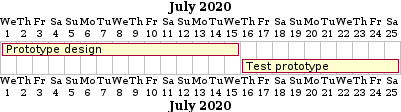
\includegraphics[width=0.6\linewidth]{Images/Diagrams/trivial_gantt.png}
    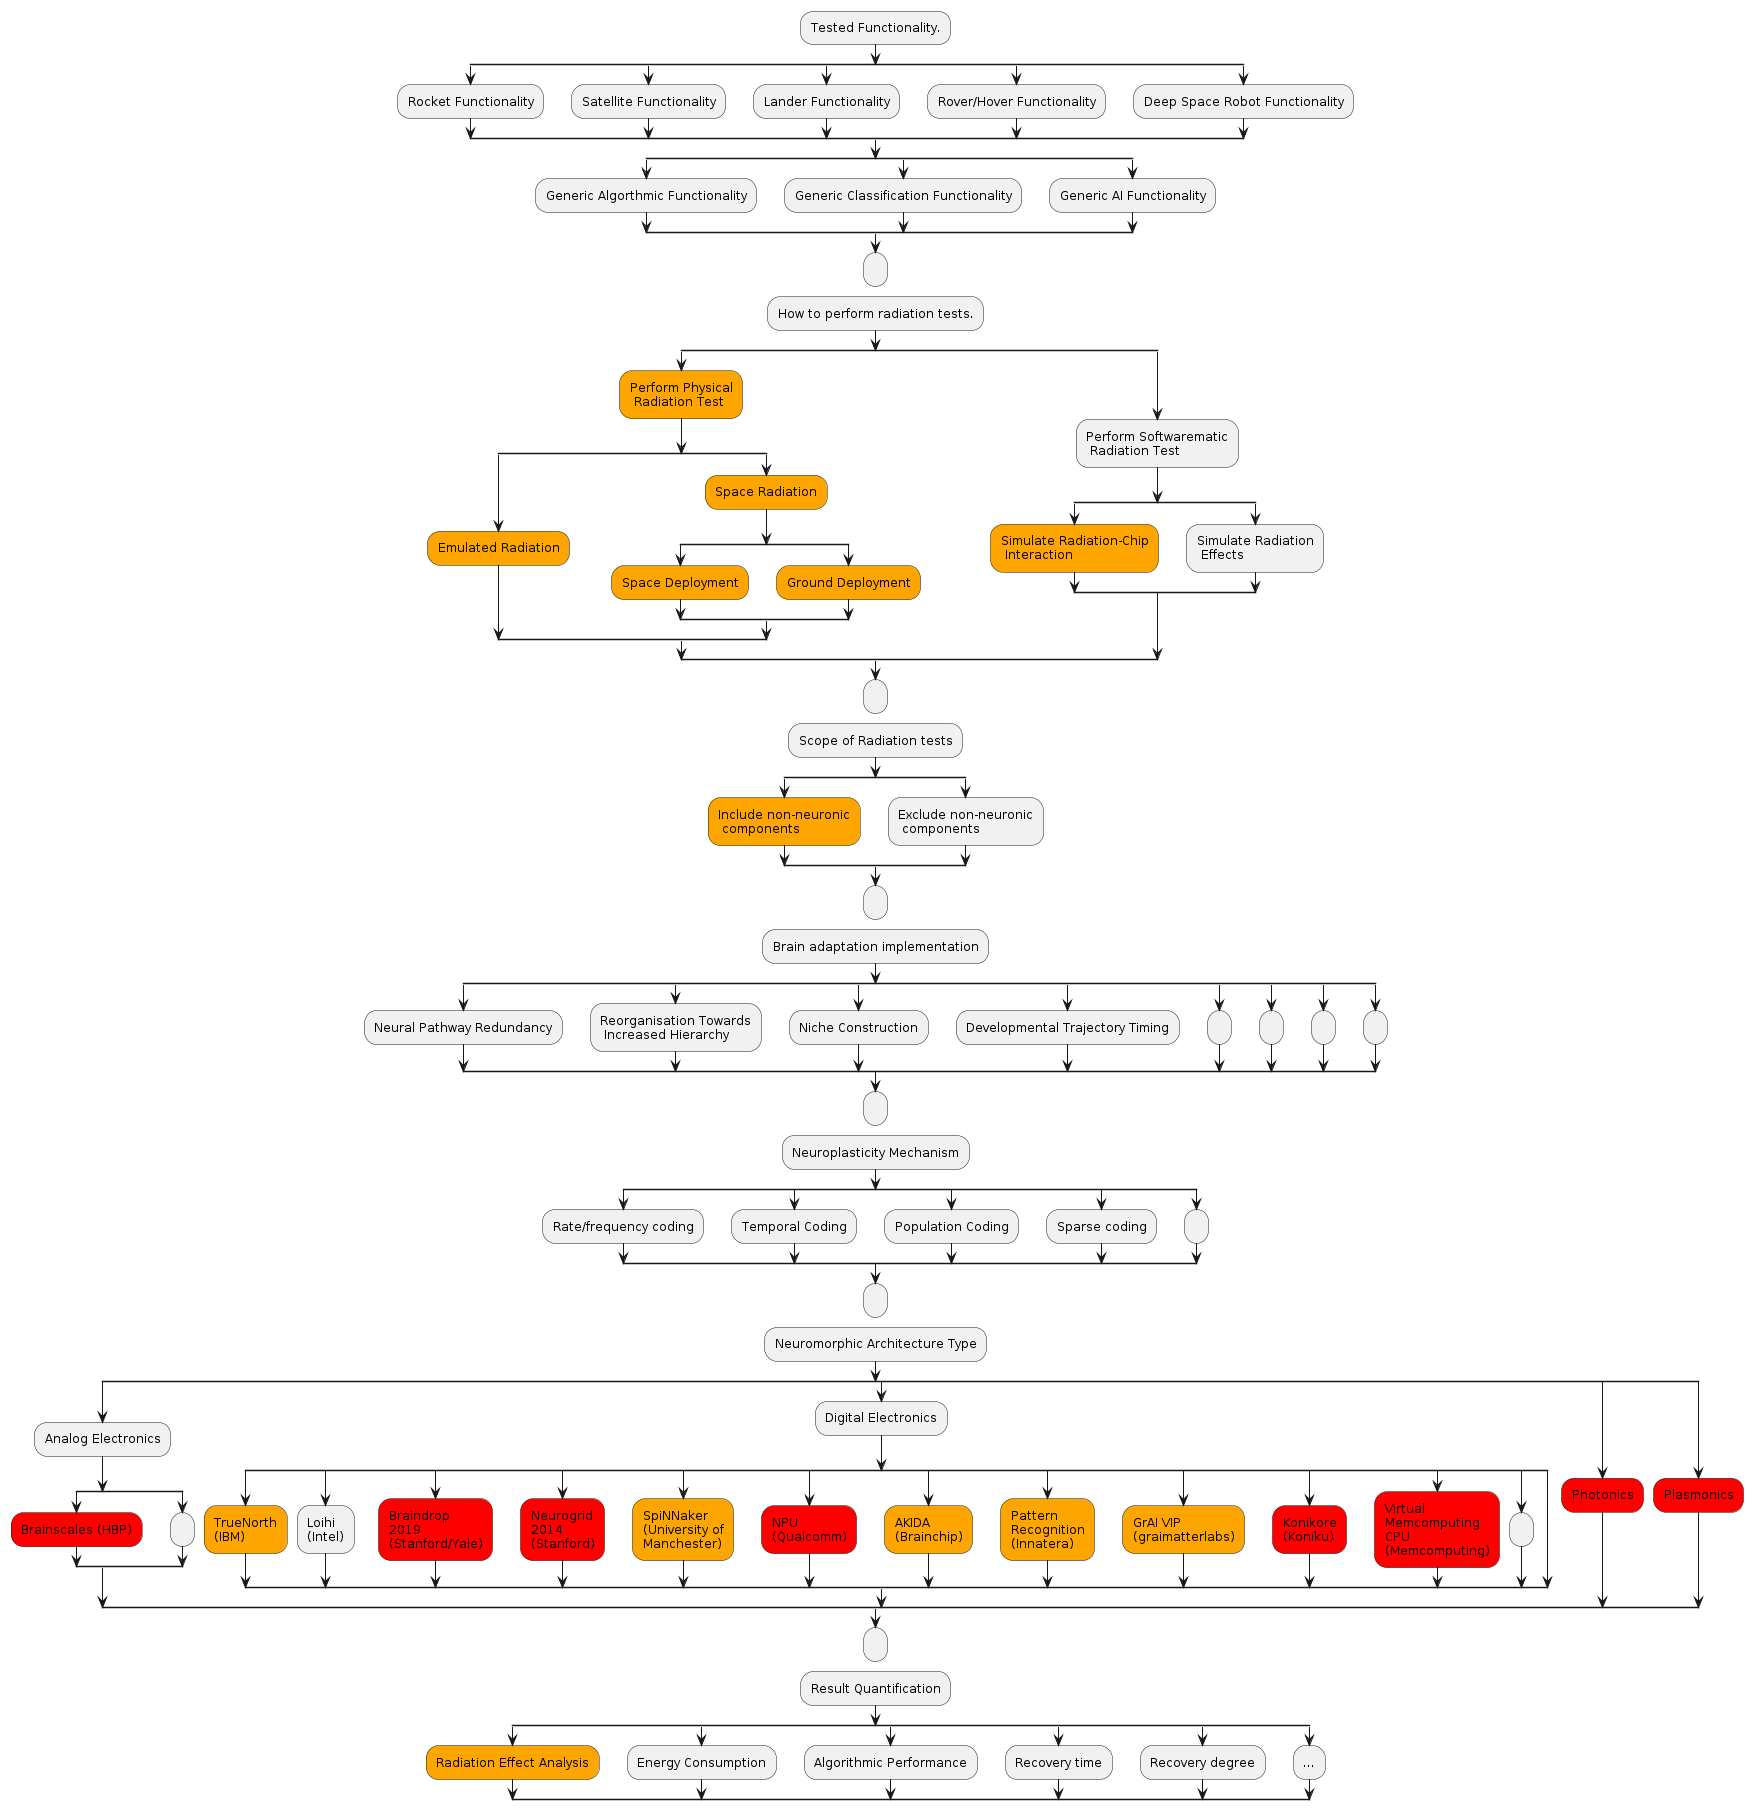
\includegraphics[width=0.6\linewidth]{code/src/Static_diagrams/dot_pruned.png}
    \caption{A functional flow diagram with the high-level functions of the system that is to be designed.}
    \label{fig:baseline_dot}
\end{figure}


\section{Preliminary Design Option Selection}\label{sec:baseline_preliminary_design_option_selection}
With some design options eliminated, an analysis can be performed to see whether some design options are considered to be more feasible than others. This analysis is started by taking the \textbf{STKH-SPACEBRAINS-01} requirement into account, which implies results need to be produced by April 15th. This allows for expressing some design option preferences as listed in \cref{subsec:baseline_tested_functionality_preference} to \cref{subsec:baseline_result_quantification_preference}. Taking the full scope of the thesis project into account allows identification of design options that seem most feasible for a follow-up with physical radiation testing.

\subsection{Tested Functionality Preference}\cref{subsec:baseline_tested_functionality_preference}
For performing a \textit{generic algorithmic functionality} for the following two reasons:
\begin{enumerate}
    \item No additional dependencies such as datasets, panda packages, tensorflow etc. is required. This lowers the probability of allocating time on work that does not directly support the objective of this thesis project.
    \item No preprocessing work, such as loading and/or cropping images etc.,  is required. This increases the amount of time that can be allocated to implementing the brain adaptation and testing its functionality.
    \item Graph algorithms are typically used in space applications \cite{todo}.%, an example is the MDS approximation in communication satellites.
    \item Thorough testing can quickly be set up for graph algorithms.
\end{enumerate}
 
\subsection{How To Perform Radiation Tests Preference}\cref{subsec:baseline_how_to_perform_radiation_tests_preference}
Using softwarematic radiation tests that simulate radiation effects.

\subsection{Scope of Radiation Tests Preference}\cref{subsec:baseline_scope_of_radiation_tests_preference}
Excluding non-neural components from radiation effects allows for a complete focus using the expected radiation effects on the neural and synaptic properties, without having to model additional radiation interactions with (other) hardware elements. This increases the feasibility of producing results by April 15th.

\subsection{Brain Adaptation Implementation Preference}\cref{subsec:baseline_brain_adaptation_implementation_preference}
No preference in brain adaptation implementations is expressed at the time of writing.

\subsection{Neuroplasticity Mechanism Preference}\cref{subsec:baseline_neuroplasticity_mechanism_preference}
No preference in neuroplasticity mechanisms is expressed at the time of writing.

\subsection{Neuromorphic Architecture Type Preference}\cref{subsec:baseline_neuromorphic_architecture_preference}
Based on availability and previous experience, a preference is expressed for the Loihi platform for the softwarematic simulation. Insights from this simulation will be used to determine the best way forward towards hardware simulations. Since the Innatera chips are expected to be available for testing in the second quarter of 2022, combined with there relatively low cost, this option is mentioned as a possible suitable candidate for physical radiation testing. The Spinnaker boards appear to have a higher unit cost.

\subsection{Result Quantification Preference}\cref{subsec:baseline_result_quantification_preference}
Based on the vicinity of the ICONS deadline of April 15th, 2022, a preference is expressed for measuring the softwarematic results in terms of algorithmic performance. This is because it forms the most direct measurement that can be used to determine whether the principle of brain adaptation is indeed able to increase the radiation robustness of neuromorphic space hardware.

\subsection{Preliminary Design Option Tree}\label{subsec:preliminary_design_option_tree}
The preferences expressed in \cref{sec:baseline_preliminary_design_option_selection} are coloured green in the preliminary design option tree visualised in \cref{fig:baseline_preliminary_dot}.

\begin{figure}[H]
    \centering
    %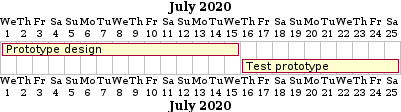
\includegraphics[width=0.6\linewidth]{Images/Diagrams/trivial_gantt.png}
    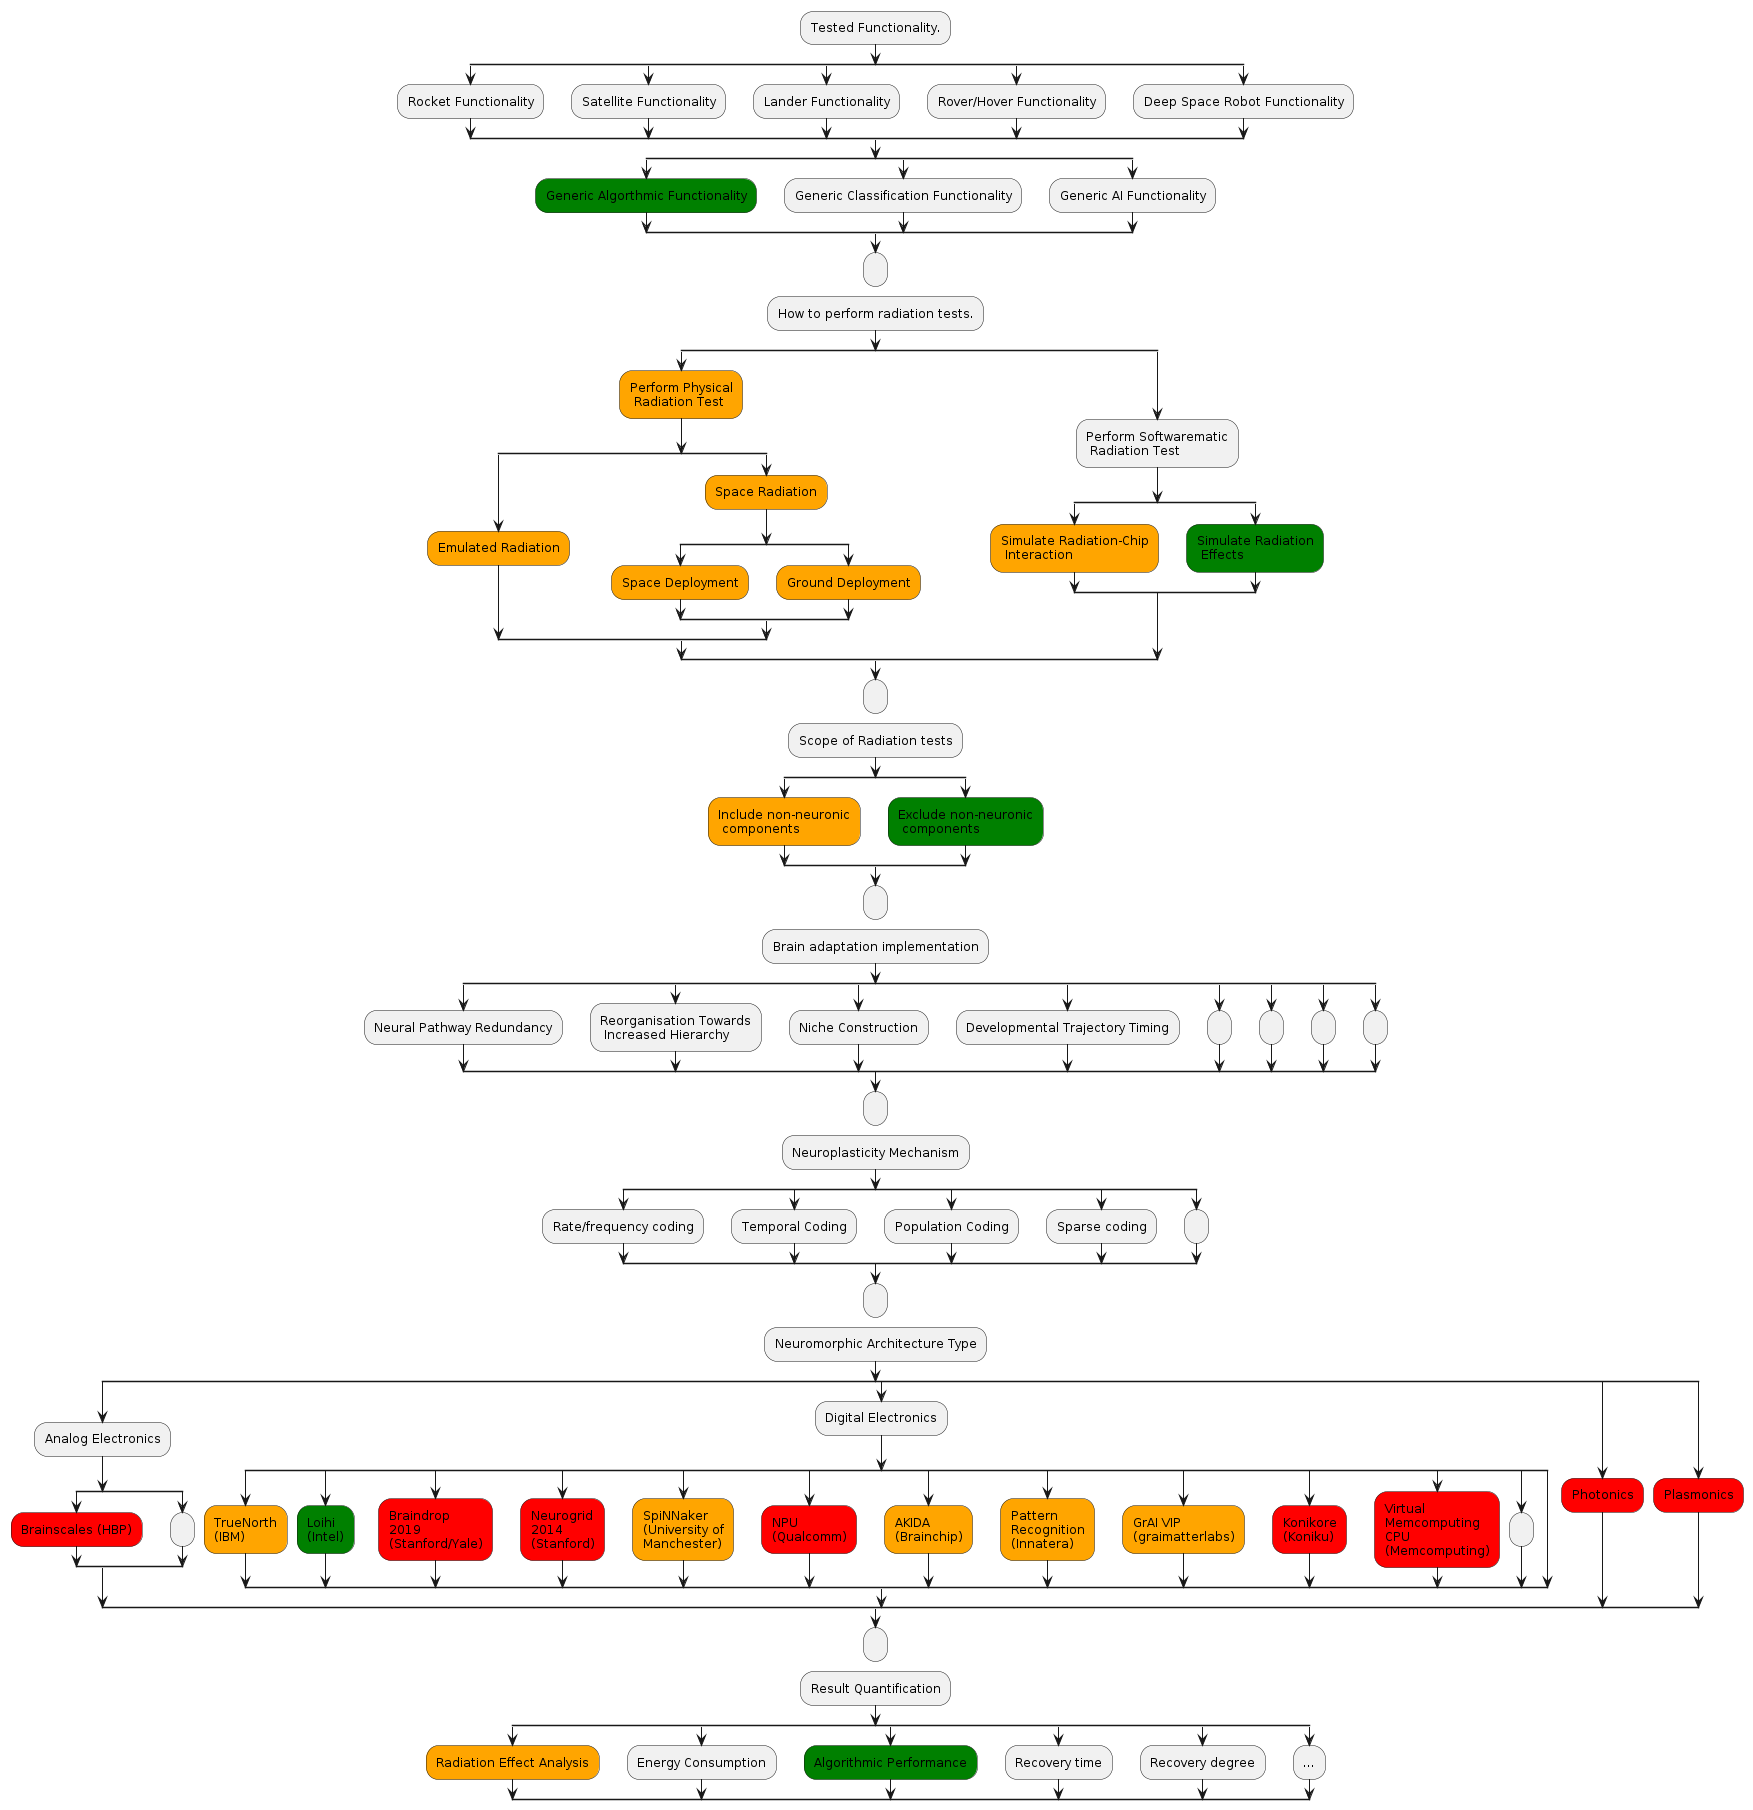
\includegraphics[width=0.6\linewidth]{latex/Images/Diagrams/Static_diagrams/dot_preliminary.png}
    \caption{todo}
    \label{fig:baseline_preliminary_dot}
\end{figure}

\section{Proposed Design options}\label{subsec:baseline_proposed_design options.}
To summarise, a distinction between project phases. First a softwarematic test is performed and the results are reported to the ICONS by  April 15th 2022. Next, a hardwarematic test is proposed that builds upon the knowledge gained in the softwarematic tests. For the first phase, the following options are proposed to be executed during the midterm: A graph algorithm is proposed to be ran, where the radiation effects on the neuromorphic architecture are simulated as changes in the the neural and synaptic properties of the spiking neural networks. For this first softwarematic test, the radiation effects on non-neural/traditional hardware components (such as a memory bus, \acrshort{cpu} etc.) of the neuromorphic architecture are ignored. The Loihi platform will be used for the simulation development and radiation tests. The test results will be interpreted in terms of performance of the graph algorithm. The most feasible brain-adaptation method and neuroplasticitiy mechanism will be determined using hands-on experimentation.
% TODO: change generic alg to graph alg
For the second tests, a physical radiation test is proposed. For this test, the Innatera chips are currently considered as the most feasible option. Based on the results of the softwarematic testing, a decision can be made to inlcude the traditional hardware components of the respective chips. An alternative option could be to apply extra shielding to those components, whilst saving mass on the non-shielded components though the use of brain adaptation inspired implementations.
